\scanpage{11}
\unsure{geometricqlly|geometrically} irreducible, i.e. $\underline{D}$ is constant, and assume $B$ geometrically regular over $k$. This second condition implies that $X\handwritten{\widehat{\otimes}}_k B$ is regular, and denoting by $U\handwritten{\widehat{\otimes}}_k B$ the inverse image of $U$ in this scheme, \deleted{the first condition} this \unsure{togetther|together} with the first condition implies that \deleted{the \deleted{\unsure{right}}\inserted{left} hand side of (20)}\inserted{\handwritten{$\operatorname{Pic}(X\widehat{\otimes}_k B)/\underline{D}(B)$}} is isomorphic to $\operatorname{Pic}(U\handwritten{\widehat{\otimes}}_k B)$. This shows that o n the sub-category of arguments $B$ which are \deleted{\unsure{ge}} noetherian and geometrically regular, $Q$ is the étale sheaf associated to the presheaf
\[
B\handwritten{\longmapsto}\operatorname{Pic}(U\handwritten{\widehat{\otimes}}_k B)\handwritten{/\operatorname{Pic}(B)}\deleted{\unsure{(}}\handwritten{(\hookrightarrow}Q(B))\ .
\tag*{(21)}
\]
The obstruction for an element of $Q(B)$ to belong to $\operatorname{Pic}(U\handwritten{\widehat{\otimes}}_k B)\inserted{\handwritten{/\operatorname{Pic}(B)}}$ is in the Brauer group $\operatorname{Br}(B)$. Thus, under very stringent conditions on $B$ at least (being geometrically regular) we get a description of $Q(B)$ in terms of actual local Picard groups. I should have stated that $U\handwritten{\widehat{\otimes}}_k B$ can also be interpreted as the inverse image of $U$ in the scheme $\unsure{\mathbb{S}|S}\mathrm{pec}(A\handwritten{\widehat{\otimes}}_k B)$, and thus makes a sense independently of the choice of a particular resolution.

One may wish to construct a local Picard scheme \deleted{without} also in case $A$ is not equi-caracteristic, which implies that $\mathrm{car}.k\handwritten{>}0$. It seems likely that this can be done if $k$ is perfect. The key-point here \deleted{seems} \deleted{to} is the construction of schemes $P_n$, which leads us to the following

\uline{$\unsure{\mathbb{P}|P|B}$roblem}\quad Let $A$ be a local Artin ring with perfect residue field $k$ of car. $p\handwritten{>}0$, $X$ a proper scheme over $A$. Give a ``natural'' construction of a group scheme locally of finite type $P$ over $k$, together with an imbedding
\margin{\figure{\handwritten{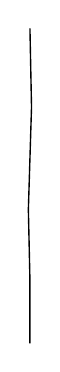
\begin{tikzpicture}\draw[line width=.5pt] (0,0)--(.02,-1)--(-.02,-2.3)--(0,-3.2)--(0,-4);\end{tikzpicture}}}}
\[
\operatorname{Pic}(X)\handwritten{\hookrightarrow}P(k)\ ,
\tag*{(22)}
\]
the obstruction for an element of $P(k)$ to beling to $\operatorname{Pic}(X)$\handwritten{(}being in $\operatorname{Br}\ H^{\unsure{o|0}}(X,\underline{O}_X)$, and hence\handwritten{)}vanishing if $k$ is algebraically \unsure{closed|closee}.
% archive sheet number: 10
